\section{实验步骤}

\subsection{模型保存}

代码包中提供的workflow示例代码会保存模型,你也可以在workflow代码中的任意时机调用agent.save\_model保存中间模型。 注意:虽然agent.save\_model接受path和id两个参数,但在分布式训练时,workflow中调用该接口传入的参数会被框架覆盖成实际的模型保存路径以及最新的训练步数。

为了避免用户保存模型的频率过于频繁,模型保存会有安全限制,限制规则如下:

\begin{enumerate}
    \item 保存模型的频率限制: 2次/分钟
    \item
    单个任务保存模型的次数限制:(不同算法的限制不同)
    DQN or Target-DQN:100次
    DIY:100次
\end{enumerate}

\subsection{评估模式}

开悟平台支持评估模式,帮助用户在训练后评估模型的能力。相比较训练时用户可以在每一局设置usr\_conf,评估时用户需要在提交任务界面进行宝箱配置。另外,训练模式时,用户一般使用agent.predict方法进行决策;而在评估模式时,平台会调用agent.exploit方法进行决策,一般情况下,模型在训练和评估时的决策会因算法不同和用户设计不同,而有不同的行为,这部分由用户定义和实现。


\subsection{代码调试}

在代码包的根目录,我们提供了代码测试脚本train\_test.py,该脚本将使用算法文件夹下train\_workflow.py中的workflow进行一次训练,当训练步数>0时判定本次代码测试通过。通过启动一次训练,脚本能够迅速验证流程中的各个环节是否正确进行,确保训练逻辑的准确性。

为避免训练模型时出现因代码问题导致的错误,我们建议你在正式训练前一定要对代码进行测试。操作如下:

\begin{enumerate}
    \item 将train\_test.py文件中algorithm\_name的值修改为需要测试的算法名,算法名需要是algorithm\_name\_list中的一个。
    
    \item 进入IDE工具栏的【运行与调试】工具,点击下图所示绿色箭头的 运行 按钮。启动后,IDE会开始对代码进行测试,并将运行结果输出到右侧面板下方的终端区域,以方便你进行观察和分析。
\end{enumerate}

\begin{figure}[H]
    \centering
    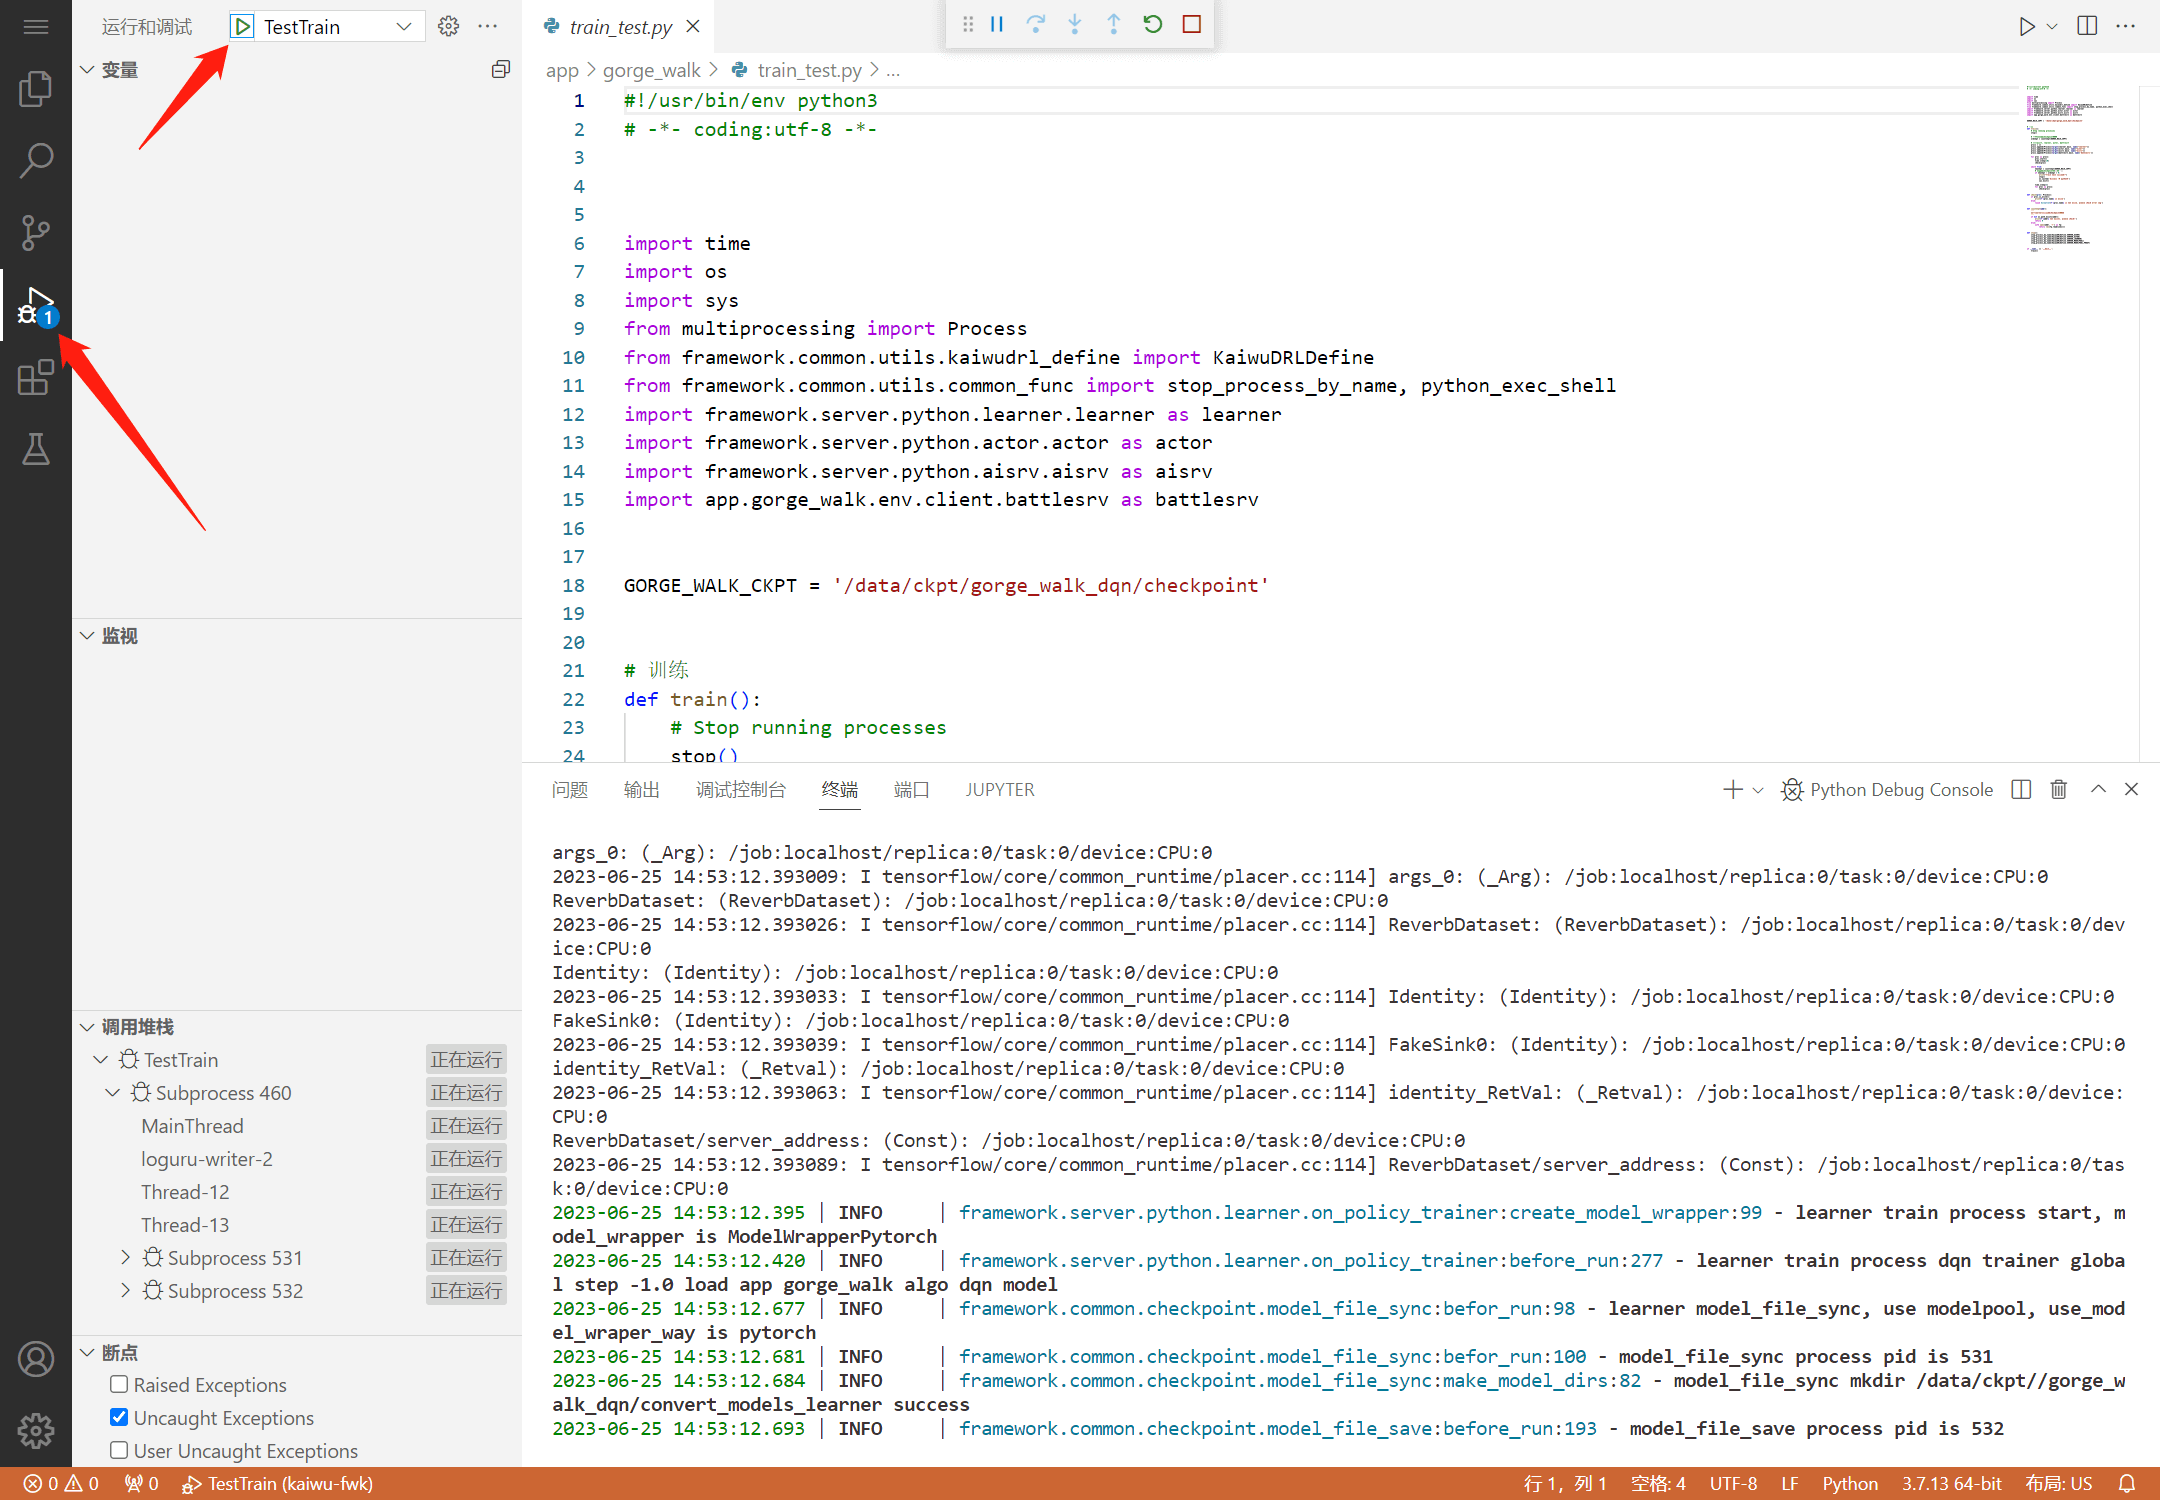
\includegraphics[width=1\linewidth]{pic/debug.png}
    \caption{\zihao{-5} 代码调试}
    \label{debug}
\end{figure}

在代码测试过程中如果遇到错误,则测试流程自动中止。此时你可以根据下方的终端面板查看错误信息,根据错误信息定位代码的问题。

如果没有遇到错误,则代码测试流程会在一次强化训练结束后自动终止(几分钟左右,请耐心等待),并在下方的终端面板提示Train test succeed。